\section{State of the art}
\label{section_sota}
Dantzig's simplex algorithm~\cite{simplex} (1947) is one of the oldest algorithms to solve linear optimization problems. Its geometric interpretation allowed the creation of a family of algorithms for the vertex enumeration problem called the pivoting algorithms~\cite{pivoting}. This section presents the required background knowledge regarding the simplex algorithm as well as one pivoting algorithm: the Avis-Fukuda algorithm~\cite{fukuda} (refereed as Fukuda's algorithm in the rest of the paper).

\subsection{The simplex algorithm}

\subsubsection{Linear optimization.}
The simplex algorithm is an algorithm that solves \emph{linear optimization problems}. A linear optimization problem is finding the maximum of a linear function (the objective) $(x_i)_{i=1}^n \mapsto \sum_{i=1}^n c_i x_i$  under a set of linear inequality constraints $\sum_{i=1}^n a_i x_i \leq b_i$. Geometrically, such a problem is to find the point which coordinates maximizes the objective, which can be seen as a direction, in an area defined by a set of half-spaces (each constraint is the equation of a half-spaces).

The set of the points respecting all the constraints is called the feasible area. To simplify the problem, the origin is assumed to be in the feasible area (equivalently: all the $b_i$ are positive) and the feasible area is assumed to be contained in $(\mathbb{R}_+)^d$. When a point is on a constraint (its coordinates turn the inequality into an equality), the constraint is called \emph{saturated}. 

The first step of the algorithm is to turn all the inequalities into equalities by the addition of positive \emph{slack} variables. These variables correspond to a distance from the associated constraint. Note that every variable (slack or not) corresponds to a constraint and thus to a half-space. Assigning a variable to a negative value means violating the corresponding constraint. In the following, the non-slack variables will be referred as \emph{original}.

\subsubsection{The dictionary.}
By adding to these equalities an other equality corresponding to the cost function, a tableau of coefficients is obtained. This tableau is called a dictionary. So far, every row corresponds to a slack variable plus one for the objective function and every column corresponds to an initial variable, plus one for the constants. In the rest of this report, the entry in the row $i$ and column $j$ is named $a_{ij}$.


The dictionary allows to find the value of every variable knowing the value of those associated to the columns. The set of the variables associated to the columns is called the \emph{cobasis}, the set of the variables associated to the row is called the \emph{basis}. Setting all the variables of the cobasis to zero provides a valuation for all the original variables. Such valuation describes a point against $d$ hyperplanes: a vertex of the hyperplane arrangement.% The cobasis is a coordinate system composed by the normal vectors of the hyperplanes associated to the variables in the cobasis, with for origin point the intersection of these hyperplanes.
In the following, the basis is called $B$, the cobasis $N$, the row corresponding to the objective function is $f$ ($\in B$) and the column containing the constants is $g$ ($\in N$).  

\subsubsection{The pivot.} 
The idea of the simplex is to exchange the variables between the basis and the cobasis (and updating in consequence the coefficients of the dictionary) such that when the cobasis is set to zero, the objective function increases and no basic variable is set to a negative value. This operation is called a pivot. From a geometrical point of view this operations consist in keeping $d-1$ constraints saturated and exchanging the remaining one for an other.%, increasing the objective and staying in the feasible area..
The vertices of the feasible area are explored until a maximum is reached. For a pivot occuring between the variables $r$ and $s$, $a_{rs}$ is refereed as the coefficient corresponding to the pivot. If it equals zero, the pivot is impossible and it means that the variable of the basis is independent from the variable from the cobasis. The most spread rule to select the pivot of a dictionary is Bland's rule~\cite{bland}, it ensures that the next dictionary describes a point in the feasible area and the termination of the algorithm.

%To maintain the fact that the cobasis expresses the vector of the basis, the following transformations are applied to the dictionary. The coefficients of the new dictionary are primed, the pivot occurs between $r \in B-f$ and $s \in N-f$ and the transformation is for all $(i,j)\in (B-r,N-s)$:
%$$ a'_{sr}=\frac{1}{a_{rs}}, \hspace{1cm} a'_{ir}=\frac{a_{is}}{a_{rs}}, \hspace{1cm} a'_{sj}=-\frac{a_{rj}}{a_{rs}}, \hspace{1cm} a'_{ij}=a_{ij}-\frac{a_{is}a_{rj}}{a_{rs}}.$$


%A major issue of the simplex is that it can loop, this is overcome with Bland's rule to pick a pivot. It ensures the termination of the algorithm and ensures the point represented by the dictionary stays inside the feasible area.

%This rules applied to the dictionary of example~\ref{lp3} calls for pivoting around the first row and the first column. Which sends $x$ to the basis and $s_1$ to the cobasis. Setting the cobasis to $0$ indicates that the dictionary represents the point $(2,0)$. The next pivoting is around the second row and the second column which leads to the point$(2,7)$, the Bland's rule then state that the optimum is reached. The example~\ref{lp4} provides the transformations of the dictionary.



\subsubsection{Some properties.}
A basic variable is primal feasible if the associated constant is non negative, a cobasic variable is said dual feasible if the associated coefficient in the objective function is non positive. A dictionary is primal (resp. dual) feasible if all the variables is the basis (resp. cobasis) are primal (resp. dual) feasible. A dictionary is optimal if it is both primal and dual feasible. A dictionary is primal feasible if and only if it describes a point inside the feasible area. A dictionary is dual feasible if and only if there is no pivot able to increase the objective.

\begin{proposition}
The normal vectors of the hyperplanes associated to the variables of the cobasis describe an independent family: the cobasis is, in fact, a basis.
\end{proposition}
\vspace*{-0.1cm}
This proposition is obtained by induction. At the beginning of the algorithm the cobasis is the canonic basis. The only operation applied to the dictionaries (the pivoting) maintain this property. If one tries to break this invariant, the new potential member of the cobasis is a linear combination of the others. This means the value of the corresponding variable is determined by the other member of cobasis which implies the pivoting provoked a division by zero.


\subsubsection{Alternative forms.}
\label{section_altsimplex}
So far, the origin is assumed to be in the feasible area and all the variables were positive. There exist alternative forms of the simplex for problems where the above assumption does not hold:

\paragraph{If the origin is not in the feasible area,} the simplex works in two phases: joining the feasible area, then optimizing. Joining the feasible area is done by an other simplex instance: 
\vspace*{-0.1cm}
\begin{itemize}
\item the constraints are the complementary half-space of each violated constraints alongside with the non violated one;
\item the function to maximize is the opposite of the sum of the slack variables corresponding to the violated constraints.
\end{itemize}
\vspace*{-0.1cm}
The simplex then continues with the initial constraints and objective function, but the current basis and cobasis.

\paragraph{If the variables are not all positive,} the idea of the simplex remains: pushing the cobasis to its bound to obtain a vertex. The sole difference is that the bounds are not $0$ anymore. Since the original variables might not be bounded, or that there might be both lower and upper bounds, a valuation for all the variables is kept (initialized at $0$ for all). The valuation is modified when a pivot occurs: the the new cobasic variable is push to its bound that maximizes the objective.


\subsubsection{An example of the simplex algorithm.} Here is given an example of use of the simplex algorithm on the linear optimization problem: maximize $x+y$ under $y\leq 2$ and $x-y\leq 2$.
\vspace*{-0.4cm}
\begin{multicols}{2}
\paragraph{Creation of the dictionary:} the slack variables are defined $0 \leq s_1 = 2-y$ and $0\leq s_2=2-x+y$. These equalities are then put together in the dictionary:
\begin{tabular}{| c | c || c || c c |}
\hline	
$x$ & $y$ & constants & & \\
$\downarrow$ &$\downarrow$ &$\downarrow$ & & \\
\hline
\hline	
$0$ & $-1$ & $2$ & = & $s_1$\\ \hline	
$-1$ & $1$ & $2$ & = & $s_2$\\ \hline \hline	
$1$ & $1$ & $0$ & $\leftarrow$ & objective function \\
\hline	
\end{tabular}

Bland's rule tells to pick $x$ and $s_2$ for the first pivot, which leads to
\begin{tabular}{| c | c || c || c c |}
\hline
$s_2$ & $y$ & const & & \\
\hline
\hline	
$0$ & $-1$ & $2$ & = & $s_1$\\ \hline	
$-1$ & $1$ & $2$ & = & $x$\\ \hline \hline	
$-1$ & $2$ & $2$ & $\leftarrow$ & obj \\
\hline	
\end{tabular}.


Then $y$ and $s_1$: 
\begin{tabular}{| c | c || c || c c |}
\hline
$s_2$ & $s_1$ & const & & \\
\hline
\hline	
$0$ & $-1$ & $2$ & = & $y$\\ \hline	
$-1$ & $-1$ & $4$ & = & $x$\\ \hline \hline	
$-1$ & $-2$ & $6$ & $\leftarrow$ & obj \\
\hline	
\end{tabular}.
There is no other pivot selected by Bland's rule, note that the final dictionary is optimal.

\columnbreak

\figurecol{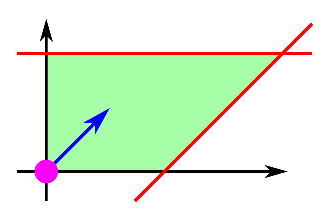
\includegraphics[width=\columnwidth]{images/simplex12.eps}%
\figcaption{Geometrical interpretation of the maximization problem. The constraints are in red, the blue arrow corresponds to the gradient of the objective function, the feasible area is shaded, the purple point is the origin (the point described by the first dictionary).}}

\figurecol{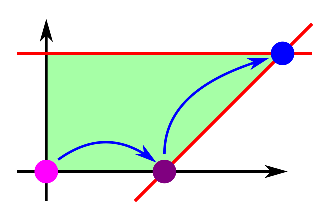
\includegraphics[width=\columnwidth]{images/simplex15.eps}%
\figcaption{The current point after the first pivot is $(2,0)$, and after the second $(4,2)$.}}



\end{multicols}























%Instead of setting the cobasis to zero, lower and/or upper bounds can be kept for each variables, alongside with a valuation (initialized at $0$ for every variable). The original variables don't have bounds. Once again the valuation of the variables of the cobasis is sufficient to determine the valuation of the basis. The dictionary stays identical (only the constants' column becomes useless). Here the variables can be positive or negative.

%The first phase will be to reach the feasible area, i.e. ensure that for all the variables, the valuation respects the bounds. To do so, let's pick a variable $i$ in the basis which bounds are not satisfied, without loss of generality let's assume the upper bound is not satisfied. Then let's pivot it with a cobasic variable $j$ smaller than its upper bound if $a_{ij}>0$ or greater than its lower bound if $a_{ij}<0$. Then the variable $i$ is assigned to its upper bound and the new valuation of the basis is computed. This operation is to be repeated until all the variables are in their bounds, a feasible point is found, or until no suitable pivot can be found, the feasible area is empty.

%The second phase, the optimization is very similar to the classic algorithm, instead of pushing the cobasis to zero, the valuation is fixed and the variables are pushed to their upper or lower bound (depending on the objective) when they are sent in the cobasis. This second phase will not be used in this paper.






\subsection{Fukuda's algorihm}

%vague overview
Fukuda's algorithm allows to enumerate all the vertices of an $\mathcal{H}$-polytope included in the positive orthant ($(\mathbb{R}_+)^d$, all its points have non-negative coordinates) for which the origin is a vertex. This algorithm uses the pivoting scheme of the simplex to explore the polytope. 

It is based on a simple idea: starting from any vertex, the simplex algorithm allows to reach a vertex maximizing a linear function by a unique (thanks to Bland's rule) path among the vertices. The algorithm picks a function maximized only by the origin on the positive orthant and walks backward on all the paths leading to it from all the vertices. Every time a vertex is encountered, it is output.

The first thing to do is to find the end of all these paths: the dictionary corresponding to the origin. It roughly consists in taking the canonical base as cobasis and the set constraints as the basis and setting $-\sum_{i=0}^d x_i$ as the cost function. All the possible pivots are tried from this dictionary. If a pivot leads to a primal feasible dictionary (defining a vertex inside the polytope) for which the Bland's method leads back to the previous point it is said to be a valid reverse Bland's pivot. It means that a step backward has been made on one of the paths, the new point is output, and the method has to be applied from this new point.

However, if a vertex is defined by more hyperplanes than required, several dictionaries will describe the same point, which is said to be degenerated. Fukuda overcomes this problem by defining a partial order on the dictionaries. This order corresponds to a lexicographic order on the basis for the dictionaries defining the same point. A point is only output if its dictionary is lexicographical minimal. Note that the algorithm continues on the dictionary, even if it is not lexicographical minimal.

If the origin is degenerated, then all the optimal dictionaries defining it have to be found. This is done by using a procedure very similar from the one above: by looking only at the hyperplanes redefining the origin, every pivot is tried. The difference is instead of using the Bland's rule, a variation of the dual Bland's rule is used. If the new dictionary is dual feasible (still an optimal for the cost function) and the dual Bland's rule brings it back to the previous one, then the new dictionary is valid with respect to the dual Bland's rule etc. This research presents the same uniqueness properties than the previous one. The previous research has to be launched from every dictionary obtained this way.

The following example illustrates Fukuda's algorithm on a polytope with no degenerated vertex:

\begin{example}
	Let $h$ be the polytope included in the positive orthant and the half-space $x+2y\leq 4$ (plus the positive orthant, i.e. $-x\leq 0$ and $-y\leq 0$) in $\mathbb{R}^2$.\\
	First step, the optimal dictionary:
	\begin{tabular}{| c | c || c || c c |}
	\hline	
	$x$ & $y$ & const & & \\
	$\downarrow$ &$\downarrow$ &$\downarrow$ & & \\
	\hline
	\hline	
   	$-1$ & $-2$ & $4$ & = & $s_1$\\ \hline \hline	
   	$-1$ & $-1$ & $0$ & $\leftarrow$ & obj \\
   	\hline	
 	\end{tabular}, 
 	$(x,s_1)$ and $(y,s_1)$ are both valid reverse Bland's pivot and gives respectively:
 	\begin{tabular}{| c | c || c || c c |}
	\hline	
	$s_1$ & $y$ & const & & \\
	$\downarrow$ &$\downarrow$ &$\downarrow$ & & \\
	\hline
	\hline	
   	$-1$ & $-2$ & $4$ & = & $x$\\ \hline \hline	
   	$1$ & $1$ & $-4$ & $\leftarrow$ & obj \\
   	\hline	
 	\end{tabular}
 	for the point $(4,0)$ and
 	\begin{tabular}{| c | c || c || c c |}
	\hline	
	$x$ & $s_1$ & const & & \\
	$\downarrow$ &$\downarrow$ &$\downarrow$ & & \\
	\hline
	\hline	
   	$-\frac{1}{2}$ & $-\frac{1}{2}$ & $2$ & = & $y$\\ \hline \hline	
   	$-\frac{1}{2}$ & $-\frac{1}{2}$ & $-2$ & $\leftarrow$ & obj \\
   	\hline	
 	\end{tabular}
 	for the point $(0,2)$. These two dictionaries have no valid reverse Bland's pivot, the enumeration is done.
	\label{example-fukuda}
\end{example}

\paragraph{Complexity:} for $n$ half-space in a space of dimension $d$, Fukuda gives a complexity of $O(nd(n+d)g)$, where $g$ is the number of vertices of the polyhedron, counted with their multiplicity (a degenerated vertex can be define in several ways, it is counted several times). 